\documentclass[a4paper, 11pt]{article}
% For UTF-8 encoding
\usepackage[utf8]{inputenc}
% For proper hyphenation etc.
\usepackage{babel}
% For clickable links
\usepackage{hyperref}
% Set page margins
\usepackage[top=2cm, bottom=2cm, left=2.5cm, right=2.5cm]{geometry}
\usepackage{amssymb}
\usepackage{amsmath}
\usepackage{tikz}
\usepackage{pgfplots}
\usetikzlibrary{calc,shadings}
\usetikzlibrary{positioning}
\usepackage{amsthm}
\usepackage{color}
\usepackage{algorithm,algorithmic}

%Definitions
\newtheorem{mydef}{Definition}
\newtheorem*{remark}{Remark}
\newtheorem{example}{Example}
\newtheorem{lemma}{Lemma}
\newtheorem{theorem}{Theorem}
\newtheorem{corollary}{Corollary}
\newtheorem{satz}{Satz}

\makeatletter
\renewenvironment{quotation}
{\list{}{\listparindent=1.5em
		\itemindent=0pt
		\parsep\z@ \@plus\p@}%
	\item\relax}
{\endlist}
\makeatother

\newenvironment{customlegend}[1][]{%
	\begingroup
	% inits/clears the lists (which might be populated from previous
	% axes):
	\csname pgfplots@init@cleared@structures\endcsname
	\pgfplotsset{#1}%
}{%
	% draws the legend:
	\csname pgfplots@createlegend\endcsname
	\endgroup
}%

%definitions
\def\addlegendimage{\csname pgfplots@addlegendimage\endcsname}
% definition to insert numbers
\pgfkeys{/pgfplots/number in legend/.style={%
		/pgfplots/legend image code/.code={%
			\node at (0.295,-0.0225){#1};
		},%
	},
}


%opening
%\title{	Proseminar \glqq Theoretische Informatik\grqq{}\\
%		Lineare Optimierungsprobleme und deren Lösung mit Hilfe des \textsc{Simplex}-Verfahrens}
%\author{Tilman Hinnerichs}
%\date{Sommersemester 2018}

\usepackage{fancyhdr}

\newcommand{\HRule}[1]{\rule{\linewidth}{#1}}
\setcounter{tocdepth}{5}
\setcounter{secnumdepth}{5}

%-------------------------------------------------------------------------------
% TITLE PAGE
%-------------------------------------------------------------------------------

\begin{document}
	
	\title{ \normalsize \textsc{Seminar: Selected Topics in Logic and Verification }
		\\ [2.0cm]
		\HRule{0.5pt} \\
		\LARGE \textbf{\uppercase{A Summary on:\\
			A Pivoting Algorithm for Convex Hulls and Vertex Enumeration of Arrangements and Polyhedra}
		\HRule{1pt} \\ [0.5cm]
		\normalsize \today \vspace*{5\baselineskip}}
	
	\date{Summer semester 2020}
	
	\author{
		Tilman Hinnerichs \\
		Matrikelnummer: 4643427 \\ 
		Technische Universität Dresden\vspace{1cm}\\
		Tutor: Dr. Florian Funke }}
\maketitle
\newpage
\begin{abstract}
	
\end{abstract}

\tableofcontents

\newpage

\begin{itemize}
	\item What audience? students with simple to no prior knowledge
	\item Don't just formulate presentation in words $\rightarrow$ add more stuff from paper
	\item add facet enumeration
	\item future work $\rightarrow$ paper citing this paper
	\item rewrite their definitions with yours for extra points
	\item add some of the theorems from the Simplex summary
\end{itemize}

This is a summary of the approach from Avis and Fukuda to the Vertex Enumeration problem mollified with various references to basic concepts such as the \textsc{Simplex} algorithm.  

\section{General remarks on the paper}
The paper \glqq A Pivoting Algorithm for Convex Hulls and Vertex Enumeration of Arrangements and Polyhedra\grqq{} was written by David Avis and Komei Fukuda. It was published in 1992 in the journal \glqq Discrete \& Computational Geometry\grqq{} and is regarded as one of the most cited papers in this very field with a number of 751 citations (as of 26.09.2020, according to Google Scholar). As a non-book, non-survey paper publication in such a specific field of research, this can be considered a fairly high amount of citations. 

\section{Polyhedra and Arrangements}
In this first section we will introduce the needed notations and basics for the Vertex Enumeration Problem (VEP). At first, we will have to clarify the terms and concepts of the \textit{vertex} and \textit{polyhedra}.

\begin{mydef}(Polyhedron)\\
	Given a matrix $A=(a_{ij}) \in \mathbb{R}^{m\times n}$ and a vector $b \in \mathbb{R}^m$.\\
	
	A \textit{convex polyhedron} $G$ is defined as
	\begin{equation}
		G = \{ x\in \mathbb{R}^n: Ax+b\geq 0 \}
	\end{equation}
\end{mydef}
\begin{remark}
	
	In general, this is the definition of a polytope, as polyhedra are the 3-dimensional special case of a polytope. As Avis and Fukuda use these terms interchangeably, we will do so as well in the following. 
\end{remark}

This definition states that the set of points is constrained by a set of $m$ linear inequalities with $n$ that are basically hyperplanes in the \textit{n} dimensional space. In the following we will abbreviate a \textit{convex polyhedron} simply as a \textit{polyhedron}. \\

An \textit{arrangement of hyperplanes} or \textit{arrangement} for short, is a decomposition of the given underlying space using a set of hyperplanes/ linear inequalities. As both concepts are fairly similar, we will not explicitly list \textit{arrangements} in every definition, as every following statement holds for both polyhedra and arrangements. If that is not the case, arrangements will be named separately.\\

As the convex property is crucial for this approach to work, we will define it using convex combinations.
\begin{mydef}(Convex combination)\\
	
	Let $x_1, x_2, \dots, x_n$ be a finite set of points. A convex combination is a point of the form 
	\begin{equation*}
		y = a_1x_1 + a_2x_2 + \dots + a_nx_n
	\end{equation*}
	while $a_1, \dots, a_n\in\mathbb{R^+}$, and
	\begin{equation*}
		a_1 + \dots + a_n = 1
	\end{equation*}
	
	A convex combination is a linear combination.
\end{mydef}
Based on this definition we can further describe the constraints to our polyhedra and arrangements.
\begin{mydef}
	A set is called \textit{convex} if it contains all convex combinations of its points.
\end{mydef}
As a polytope is in fact a set of points, too, this also applies to the polyhedra and arrangements.
\begin{mydef}
	For a given set of points, the convex hull is the set set of all convex combinations of these points.
\end{mydef}

In order to fully understand the last part of the title we additionally have to clarify the term \textit{vertex}, which we do by the following definition.

\begin{mydef}(Vertex)\\
	A point $v\in G$ is called a \textit{vertex} of any set $G$ \textbf{iff} there are no two other points $a,b\in G$ such that
	\begin{equation}
		v=\lambda_1 a + \lambda_2 b
	\end{equation}
	which is also called a \textit{convex combination} of $a,b$.
\end{mydef}

In order to make this definition a little more specific with regard to the definition of a polahedron, we will introduce our first corollary.

\begin{corollary}\label{corollary1}\cite{introtoAlg}\\
	A point $v\in G$ is a \textit{vertex} of $G$ \textbf{iff} it is the unique solution to a subset of $m$ inequalities solved as equations. 
\end{corollary}

\section{The Vertex Enumeration Problem}
\subsection{Definition and general remarks}
We are now ready to introduce the VEP itself with the following definition.
\begin{mydef}(Vertex Enumeration Problem)\\
	For a given polytope/polyhedron or hyperplane arrangement $G$ determine all vertices of the object given its formal representation. 
\end{mydef}

\begin{theorem}(Complexity of the VEP)\\
	The VEP is NP-hard for unbounded polyhedra.\cite{Khachiyan}
\end{theorem}


The VEP is dual to the \textit{Facet Enumeration problem}(FEP), that is finding all facets of a convex hull for a given set of points. The solution to the dual problem also yields the solution to the primal problem, too. We will introduce the term of duality in the following chapter.\\

While these recent definitions lack the ability to intrinsically motivate the applicability of this very problem, we will introduce a fairly simple example, which was taken and simplified from Avis' lecture notes.
\begin{example}(All meals for 1 Euro)\\
	Lets assume you are on a diet and additionally quite poor or minimalistic. Thus, you would like to plan your future meals, such that they only contain 3 different ingredients. Additionally, we would love to have sufficient nutrition intake, where we will only consider energy, protein and calcium intake.\\
	Our decision is also constrained by the fact that we will only have 1 Euro per day, and can also endure just up to a certain amount of each ingredient, in order not just eat dry oatmeal all day long.\\
	The values describing our problem are given in the following table:\\
	\begingroup
	\def\arraystretch{1.5}
	\begin{tabular}{|p{0.5cm}|l|p{2cm}|p{1.5cm}|p{1.5cm}|p{1.5cm}|p{2cm}|}
		\hline
		Var&Food type&Energy (kcal/100g)&Protein (g)&Calcium (mg)&Price (Euro cents)&Maximum\\
		\hline
		$x_1$&Oatmeal\footnote{Regular LIDL oatmeal}&250&15&40&10&500g\\
		$x_2$&Milk\footnote{Regular Bio LIDL milk}&80&4&130&4&1000g\\
		$x_3$&DD Stollen\footnote{https://fddb.info}&340&7&30&20&200g\\
		\hline
		&\textbf{Min. daily}&\textbf{2000}&\textbf{55}&\textbf{800}&&\\
		\hline
	\end{tabular}
	\endgroup\\
	
	The variables $x_1, x_2, x_3$ each denote the amount of each ingredient in 100g.
\end{example}

By solving the VEP, we yield all vertices of the corresponding polyhedron, that is all points that cannot be written as convex combinations of two other points. Inverting this very statement, all other points within $P$ are convex combinations of at least two other points. More specifically we are able to rewrite each point within $P$ as convex combinations of vertices of $P$. Thus, if we find all vertices of the given arrangement of linear inequalities, we can produce infinitely many food combinations by randomly choosing a convex combinations of the given vertices. However, we still have to find these vertices.

\subsection{Types of approaches}
In history there have been various approaches to the VEP, that can be classified into two categories. First, there are the so called \textit{Pivot based} methods, where this very method can be placed, too. These methods rely on traversing along the vertices using so called \textsc{Simplex} tableaus, which we will introduce in the following chapter. These approaches are mostly based on solving corresponding linear optimization problems.\\

The other method is called \textit{Fourier-Motzkin} or \textit{double description} method\cite{Motzkin}. These methods yield the vertices by successively adding hyperplanes and keeping track of the remaining possible vertices. The double description method in fact solves the dual problem of FEP. \\

While this classification was made in 1992 within this very publication, there haven't been exceptions to this ever since. We will discuss this in more detail in the last chapter.

\section{Linear Programs}
\subsection{What is a Linear Optimization Problem?}
While linear optimization problems are in general not necessary in order to solve the VEP with a pivot based method, it was utilized for this very approach. Additionally it gives us the chance to discuss and introduce some definitions and theorems that underline its simplicity and effectiveness. In the following we will use the terms \textit{linear program}(LP) and \textit{linear optimization problem} interchangeably.\\

\begin{mydef}
	Let $ G \subseteq \mathbb{R}^n$ be a polyhedron and $ c \in \mathbb{R}^n$. Then a problem of the form \\
	\vspace{0.15cm}
	\begin{quotation}
		$ z = f(x) = c^T \cdot x \rightarrow min\hspace{1cm} with\ x \in G$
	\end{quotation} 
	is called a \emph{linear} optimization problem.
\end{mydef}

Hereby $P$ describes the feasible space as a set of $n$-dimensional vectors, while the objective function is denoted with $f:P\rightarrow\mathbb{R}$, which maps the vectors into the real numbers. Additionally, we can easily see the type of optimization, here minimization, while also a maximization problem is possible. Without loss of generality we will only consider minimization problems here. The linearity of the problem is derived from the linearity of the objective function itself. \\

Furthermore, we are able to bring in a statement about the \textit{standard form} of linear programs. \\
\begin{corollary}
	All finite dim. linear optimization problems can be written in the following form:\\
	\begin{equation}
		\label{standardform}
		z = f(x) = c^T \cdot x \rightarrow min \hspace{1cm} with\ x \in G:=\{x \in \mathbb{R}^n: Ax \geq b, x \geq 0\}
	\end{equation}
	with $A\in \mathbb{R}^{m\times n}$, $b\in\mathbb{R}^m$, $x\geq 0$. Additionally, let $rank(A)=m$ and $m< n$.\\
	We call this form the \textit{standard form}.
\end{corollary}
The finite dimensionality is expressed with regard to the amount of variables, and thus the width of both objective function and coefficient matrix. \\

Hereby, the notation $x\geq0$ with $x\in \mathbb{R}$ describes the expression $x_j\geq 0$ for every $j=1,2,\dots,n$.\\ 
Please note that we naturally do not have any objective function in the original VEP formulation. For now, lets assume that we do have a any linear objective function $f$ given. We will discuss this issue in further detail later on.\\
After this quick introduction into the field of linear programs, we will now explore their solutions and the existence of those. We will use the following terminology.

\begin{mydef}
	Let $\bar{X} \in \mathbb{R}^n$ be a solution to a linear program in standard form \ref{standardform}.\\
	\begin{itemize}
		\item[(1)] If $\bar{x}$ satisfies the linear equality system defined by $A\bar{x}\geq b, \bar{x}\geq 0$ (see \ref{standardform}), we call $x\bar{x}$ as a \emph{feasible solution}. Otherwise we will call $\bar{x}$ a infeasible solution.
		\item[(2)] $\bar{x}$ is \emph{optimal}, if for its objective value $\bar{z} = f(\bar{x})$ with objective function $f$ the following applies:
		\begin{quotation}
			$\bar{z} = f(\bar{x}) \leq z = f(x)$ for all $x\in G$
		\end{quotation}
	\end{itemize}
	If a linear program has a feasible solution but no optimal one, we will call t his LP unbounded.
\end{mydef}

\subsection{Duality of LP}
Linear programs can be reformulated, by basically \glqq swapping\grqq{} the coefficient matrix, therefor introducing new variables and reformulating the linear inequalities. We will not go into further details here, as we are just interested in the yielded results. At first glance, the original or \textit{primal} inequality system and its dual formulation have not that much in common, but in fact they share and mutually propagate many interesting properties. \\

The first property to be mentioned here is their reciprocal bound, as the weak duality theorem states.
\begin{theorem}(Weak Duality Theorem)\\
	Given 
	\begin{itemize}
		\item a primal LP $(P)$ defined by $c^T\cdot x \rightarrow \min$ with $Ax\geq b, x\geq 0$, and
		\item its dual LP $(D)$ defined by $b^T\cdot u \rightarrow \max$ with $A^Tu\leq c, u\geq 0$.
	\end{itemize} 
	Let $x$ be feasible for $(P)$ and $u$ feasible for $(D)$. Then
	\begin{equation*}
		b^T\cdot u \leq c^T\cdot x
	\end{equation*}
	holds.
\end{theorem}
This law states, that any feasible solution of $(P)$ will always be larger or equal to any feasible solution of $(D)$.\\
We can proof an even stricter bound for both LPs.
\begin{theorem}(Strong Duality Theorem)\\
	The LP $(P)$ is solvable iff its dual LP $(D)$ is solvable. For an optimal solution $\bar{x}$ of $(P)$ and $\bar{u}$ of $(D)$
	\begin{equation*}
		b^T\cdot \bar{u}= c^T\cdot \bar{x}
	\end{equation*}
	holds, i.e. equality of the optimal solutions.
\end{theorem}

These theorems will help us better understand the eventual algorithm and its feasibility.

\section{Simplex algorithm}
\subsection{Calculating a first Simplex tableau from the Standard Form}
Before we are able to start applying the Simplex algorithm to a LP we need to transform it to a viable form for the procedure. Thus, we will transform a LP in the standard form into a so called \textit{Simplex tableau}. 
\begin{mydef}(Simplex tableau)\\
	A LP of the form
	\begin{equation}
		\label{tableau definition}
		z = f'(x') = c'^T \cdot x' \rightarrow min
		\hspace{1cm} \text{with}\ x' \in G':=\{ x' \in \mathbb{R}^{n+m}: A'x' = b, x' \geq 0\}
	\end{equation}
	\begin{quotation}
		\begin{tabular}{rl}
			with &$ A'\in \mathbb{R}^{m\times (m+n)} $\\
			&$ b\in \mathbb{R}^m $
		\end{tabular}
	\end{quotation}
	is called a \emph{Simplex tableau}.
\end{mydef}

In contrast to the standard form the feasible space is now restricted by linear equations rather than inequalities. Additionally the dimensionality of $x'$ has changed to $m+n$. These rather absurd looking changes are motivated by introducing so called \textit{slack variables} that are added to the smaller side of the inequality. We thus introduce a new variable $s\geq 0$ for each inequality that describes the difference of both sides. For example we can transform the inequality $x\leq y$ to the equation $x + s=y$. This new equation is equivalent in meaning to its predecessor inequality.\\

\begin{example}
	As our introductory example is way too large to efficiently show the power of the Simplex algorithm, we will reduce this problem to two variables and two new inequalities as listed below. This is already given in standard form.\\
	
	\begin{equation}
		\begin{tabular}{rrrrrrr}
			$ -z $&$=$& $-30a$ &$- $&$45b$ &$\rightarrow$& $\textbf{min}$ \\
			\\
			with&&$4a$ &$+$&$3b$&$\leq$&$100$\\
			&&$a$ & $+$&$2b$&$\leq$&$50$\\
			&&$a$ & ,&$b$ &$\geq$&$0$
		\end{tabular}
	\end{equation}
	Which we will now transform to a Simplex tableau.
	\begin{equation}
		\begin{tabular}{rrrrrrrrr}
			$ -z $&$=$& $-30x_1$ &$-$&$45x_2$ &$\rightarrow$& \textbf{$min$}&& \vspace{0.15cm}\\
			with &&$-4x_1$ &$-$&$3x_2$&$=$&$-100$&$+$&$s_1$\\
			&&$-x_1$ & $-$&$2x_2$&$=$&$-50$&$+$&$s_2$\\
			&&$x_1$ &, &$x_2$&$\geq$&$0$ &,&$s_1, s_2 \geq 0$
		\end{tabular}
	\end{equation}

	From now on we will also rename $s_1,s_2$ to $x_3, x_4$.
	\begin{equation}
		\begin{tabular}{rrrrrrrrr}
			$ -z $&$=$& $-30x_1$ &$-$&$45x_2$ &$\rightarrow$& \textbf{$min$}&& \vspace{0.15cm}\\
			with &&$-4x_1$ &$-$&$3x_2$&$=$&$-100$&$+$&$x_3$\\
			&&$-x_1$ & $-$&$2x_2$&$=$&$-50$&$+$&$x_4$\\
			&&$x_1$ &, &$x_2$&$\geq$&$0$ &,&$x_3, x_4 \geq 0$
		\end{tabular}
	\end{equation}
\end{example}

At this stage we will introduce the terms \textit{basic solution} and \textit{basic variables}. Let $I=\{1,\dots,m+n\}$ be the index set denoting the given indices in the Simplex tableau. As $rank(A)=m$ holds, $rank(A')=m$ follows, and therefor there has to be subset $I_B \subset I$ with $|I_B| = m$, such that the columns $A^i, i\in I_B$ with $A^i$ denoting the $i$-th column, are linearly independent. We hence denote $I_B$ as the \textit{basis index set} describing the \textit{basic variables} $x_B$, and the \textit{non-basis index set} $I_N=I\backslash I_B$ describing the \textit{non-basic variables} $x_N$.\\

A basic solution is defined with respect to the given equation system as a unique solution to a subset of $m$ inequalities solved as equations. This definition is similar to the characterization of corollary \ref{corollary1}. In fact, this corollary is derived from the relation of basic solutions and vertex, such that each vertex has at least one basic solution. Thus, we will now use these terms interchangeably.

\subsection{The Simplex Algorithm}
The Simplex algorithm can be divided into two phases.
\begin{algorithm}[H]
	\caption{The \textsc{Simplex} algorithm}
	\label{alg:seq}
	\begin{algorithmic}[1]
		\STATE Determine a first feasible solution (vertex)
		\STATE Determine the optimal solution
	\end{algorithmic}
\end{algorithm}

The algorithm starts by determining a first feasible solution, which is a vertex of our feasible polytope and thus a basic solution. It then iterates over all vertices in the feasible direction of the objective function.

\begin{lemma}
	If $G'\neq\emptyset$, then $G'$ has at least one vertex and at most finitely many vertices.
\end{lemma}

Thus, we should be able to find a first feasible basic solution.



\subsubsection{Phase 1: Determine a first feasible solution (vertex)}
Finding a first can be both really easy and hard. In general a first basic solution can be obtained by 
\begin{equation*}
	x' \longleftrightarrow 
	\left( \begin{array}{c}
		x_B \\ x_N
	\end{array}\right) = \left(\begin{array}{c}
		p \\ 0
	\end{array}\right) = \left(\begin{array}{c}
		A_B^{-1}\cdot b \\ 0
	\end{array}\right)
\end{equation*}
thus setting $x_N=0$ and $x_B=p$, if that solution is feasible. However, if that is not the case, we can formulate a aid LP, given by
\begin{equation}
	\label{hilfsproblem}
	\begin{tabular}{cl}
		&$h = e^T\cdot y \rightarrow min$\vspace{0.25cm}\\
		with&$y+Ax = b$,\\
		&$x, y\geq 0,$\\
		&$x\in \mathbb{R}^{(m+n)}, y\in\mathbb{R}^m$\\
		&$e= (1,\dots,1)^T\in\mathbb{R}^m$
	\end{tabular}
\end{equation}
through which we can always find a feasible basic solution if there exists one.\\
In the case of our example problem there exists a basic solution 
\begin{equation*}
	x' = \left(\begin{array}{c}
		x_1\\x_2\\x_3\\x_4
	\end{array}\right) = \left(\begin{array}{c}
		0\\0\\100\\50
	\end{array}\right)
\end{equation*}

Additionally, we can rewrite our equation system in the following form
\begin{equation*}
	\begin{tabular}{r|rr|r}
		$ST_0$&$x_1$&$x_2$&$1$\\
		\hline
		$x_3=$&$-4$&$-3$&$100$\\
		$x_4=$&$-1$&$-2$&$50$\\
		\hline
		$-z=$&$-30$&$-45$&$0$
	\end{tabular}
\end{equation*}
or in general for all LPs in form of a Simplex tableau
\begin{equation}
	\begin{tabular}{r|r|r}
		$ST_0$&$x_N$&$1$\\
		\hline
		$x_B=$&$P$&$p$\\
		&&\\
		\hline
		$z=$&$q^T$&$q_0$
	\end{tabular}
\end{equation}
as we rename all variables for the upcoming Simplex algorithm steps. We will always have the non-basic variables on top and the basic variables on the left. As we found our first feasible solution we are ready for the second phase.

\subsubsection{Phase 2: Determine the optimal solution}

For each step of the algorithm we first determine a so called \textit{Pivot element} $P_{\sigma\tau}$ by finding the column $\tau\in I_N$ chosen randomly, and the row $\sigma\in I_B$, which is determined by
\begin{equation}
	- \dfrac{p_\sigma}{P_{\sigma\tau}} := \min \left\{ -\frac{p_i}{P_{i\tau}}\ \middle|\ -\frac{p_i}{P_{i\tau}} < 0, i\in B \right\}
\end{equation} 
Hereby, we choose the row $i$ with the minimal $-\frac{p_i}{P_{i\tau}}$ and save this index to $\sigma$. The minimal quotient determines the maximum step size along the feasible direction. If $-\frac{p_i}{P_{i\tau}}\geq 0$ fir all $i$, then the original LP is unbounded and the maximum feasible step size is infinitely large. The algorithm stops in that very case. \\

If a feasible Pivot element is found the following update rules can be used, in order to obtain the new Simplex tableau. \\
\begin{quotation}
	\begingroup
	\def\arraystretch{1.5}
	\begin{tabular}{r|r|r}
		$ST_n$&$x_N$&$1$\\
		\hline
		$x_B=$&$P$&$p$\\
		\hline
		$z=$&$q^T$&$q_0$
	\end{tabular}
	$\longrightarrow$
	\begin{tabular}{r|r|r}
		$ST_{n+1}$&$x_{\bar{N}}$&$1$\\
		\hline
		$x_{\bar{B}}=$&$\bar{P}$&$\bar{p}$\\
		\hline
		$z=$&$\bar{q}^T$&$\bar{q}_0$
	\end{tabular}
	\endgroup
\end{quotation}

\begin{quotation}
	\begingroup
	\def\arraystretch{1.5}
	\begin{tabular}{lrl}
		$I_{\bar{N}} $&$:=$&$ I_N \backslash\{ \tau \} \cup \{ \sigma \}$\\
		$I_{\bar{B}} $&$:=$&$ I_B \backslash\{ \sigma \} \cup \{ \tau \}$
	\end{tabular}
	\endgroup
\end{quotation}

\begin{quotation}
	\begingroup
	\def\arraystretch{2}
	\begin{tabular}{lrll}
		$ \bar{P}_{\sigma\tau}$&$:=$&$\dfrac{1}{P_{\sigma\tau}} $&\vspace{0.1cm}\\
		$\bar{P}_{\sigma j}$&$:=$&$ -\dfrac{P_{\sigma j}}{P_{\sigma\tau}}$& $ j\in I_N\ \backslash\{\tau\}$\vspace{0.1cm}\\
		$ \bar{P}_{i\tau}$&$ :=$ & $ \dfrac{P_{i\tau}}{P_{\sigma\tau}} $&$ i\in I_B\backslash \{\sigma\}$\\
		$ \bar{p}_\sigma $&$:=$&$ -\dfrac{p_\sigma}{P_{\sigma\tau}} $&\\
		$ \bar{p}_i $&$:=$&$ p_i - \dfrac{p_\sigma}{P_{\sigma\tau}}\cdot P_{i\tau}$&$i\in I_B\backslash\{ \sigma \}$\\
		$ \bar{q}_\tau $&$:=$&$ \dfrac{q_\tau}{P_{\sigma\tau}} $&\\
		$ \bar{P}_{ij} $&$ := $&$ P_{ij} - \dfrac{P_{\sigma j}}{P_{\sigma\tau}}\cdot q_\tau$&$ i\in I_B\backslash \{\sigma\}, j\in I_N\backslash\{\tau\} $\\
		$ q_j $&$ := $&$ q_j - \dfrac{P_{\sigma j}}{P_{\sigma\tau}}\cdot q_\tau $& $ j\in I_N\backslash\{\tau\} $\\
		$ \bar{q}_0 $&$:=$&$ q_0 - \dfrac{p_\sigma}{P_{\sigma\tau}}\cdot q_\tau $ 
	\end{tabular}
	\endgroup
\end{quotation}

These are in fact just equivalent alterations of the original equation system, hereby swapping a basic and a non-basic variable. Thus, for given LP and its equation system we can uniquely determine its state by just its basic variables. 

\begin{lemma}
	A Simplex tableau and thus its solution is optimal iff $p\geq0$ and $q\geq0$
\end{lemma}

The algorithm stops with respect to the above lemma. 

The way the Simplex algorithm works can be observed in a visualization of its feasible space\ref{fig:2dvisu}. The first feasible basic solution is marked in black, the second in blue and the third in red. At first we are able to discover that the formerly mentioned quite abstract definition of a vertex corresponds to what we would also call a vertex in real life. Additionally, we can observe that the algorithm is moving along the edges of the polytope hopping from vertex to vertex along the feasible direction, defined by the objective function. \\


\begin{figure}
	\centering
	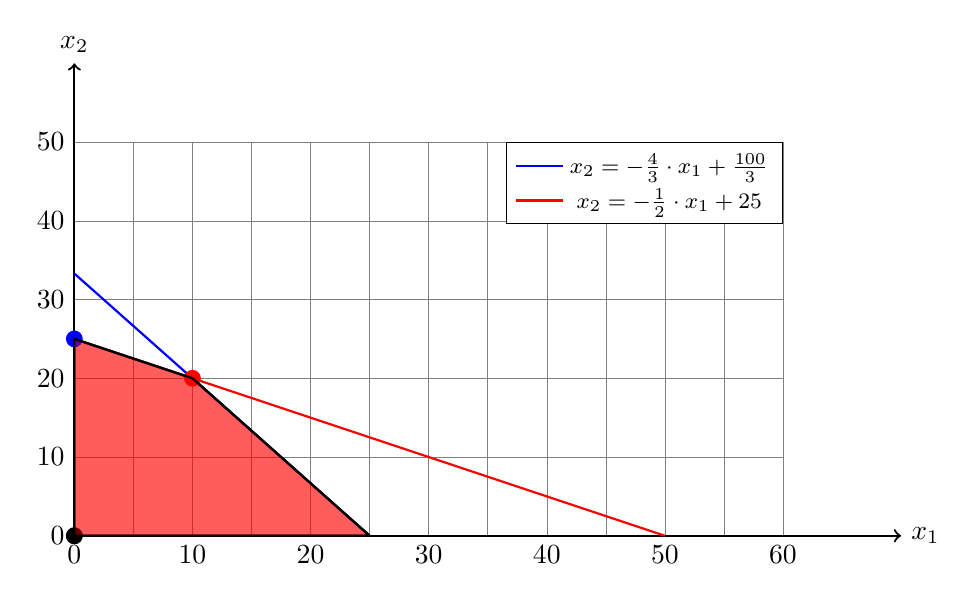
\begin{tikzpicture}[x=0.15cm,y=0.1cm]
		
		\def\xmin{0}
		\def\xmax{60}
		\def\ymin{0}
		\def\ymax{50}
		
		% grid
		\draw[style=help lines, ystep=10, xstep=5] (\xmin,\ymin) grid
		(\xmax,\ymax);
		
		% axes
		\draw[->, thick] (\xmin,\ymin) -- (\xmax+10,\ymin) node[right] {$x_1$};
		\draw[->, thick] (\xmin,\ymin) -- (\xmin,\ymax+10) node[above] {$x_2$};
		
		% xticks and yticks
		\foreach \x in {0,10,...,60}
		\node at (\x, \ymin) [below] {\x};
		\foreach \y in {0,10,...,50}
		\node at (\xmin,\y) [left] {\y};
		
		% plot the data from the file data.dat
		% smooth the curve and mark the data point with a dot
		
		% generate and plot another a curve y = 0.1 x^2 + 2.5
		% this generates the files figure.parabola.gnuplot and figure.parabola.table 
		%\draw[color=red, domain=\xmin:\xmax] plot[id=parabola]
		%function{0.1*x**2 + 2.5} node [right] {$y=0.1\,x^2 + 2.5$};
		\draw [thick, blue](0,33.3) -- (25,0) ;
		\draw [thick, red](0,25) -- (50,0) ;
		
		\node[draw,circle,inner sep=2pt,fill] at (0,0){};
		\filldraw[thick,fill=red,fill opacity=0.4] (0,0) -- (0,25) -- (10,20) -- (25,0) -- (0,0) -- cycle;
		\begin{customlegend}[
			legend entries={ % <= in the following there are the entries
				$ x_2 = -\frac{4}{3}\cdot x_1 + \frac{100}{3} $,
				$x_2 = -\frac{1}{2}\cdot x_1 + 25$
			},
			legend style={at={(60,50)},font=\footnotesize}] % <= to define position and font legend
			% the following are the "images" and numbers in the legend
			\addlegendimage{thick,blue,opacity = 1}
			\addlegendimage{thick,red,opacity = 1}
		\end{customlegend}
		\node[draw,circle,inner sep=2pt,fill] at (0,0){};
		\node[draw,circle,inner sep=2pt,fill,blue] at (0,25){};
		\node[draw,circle,inner sep=2pt,fill, red] at (10,20){};
		
		
		\filldraw[thick,fill=red,fill opacity=0.4] (0,0) -- (0,25) -- (10,20) -- (25,0) -- (0,0) -- cycle;
	\end{tikzpicture}
	\caption{Visualization of the simplified example problem}
	\label{fig:2dvisu}
\end{figure}



\begin{theorem}
	If $(P)$ is solvable, then there is a vertex of $G$ which solves $(P)$.
\end{theorem}


\subsection{The \textsc{Simplex}-Algorithm}
\begin{itemize}
	\item what does is do?
	\item How does it work
	\item why does it work? $\rightarrow$ translate some stuff from last presentation
\end{itemize}

\section{Avis and Fukudas Algorithm}
\subsection{How to move up the tree?}
Bland's rule and Criss-Cross rule
\subsection{What is it even doing?}
\subsection{Degeneracy}
with visual example from presentation
\subsection{Why is that good?}
Complexity

\section{Future Work based on this }
%body

\newpage

\begin{thebibliography}{9}
	\bibitem{introtoAlg} 
	Thomas H. Cormen, Charles E. Leiserson, Ronald L. Rivest und Clifford Stein.
	\textit{Introduction to Algorithms}. Third Edition. The MIT Press, 2009.
	\bibitem{Khachiyan}
	L. Khachiyan, E. Boros, K. Borys, K. Elbassioni, and V. Gurvich. Generating all
	verticesof a polyhedron is hard.Discrete and Computational Geometry,
	39(1):174–190, 2008.
	\bibitem{Motzkin}
	T. S. Motzkin, H. Raiffa, G. L. Thompson, and R. M. Thrall, The Double Description Method,
	Annals of Mathematical Studies, vol. 8, Princeton University Press, Princeton, N J, 1953.
\end{thebibliography}


\end{document}